\section{Background}
%I’m working on a VBF tagger
\frame {
    \frametitle{Vector Boson Fusion (VBF)}

    \begin{columns}
        \begin{column}{0.5\textwidth}
            \feynmandiagram[horizontal=a to b] {
                q1i [particle=q] -- vb1 -- q1f [particle=q],
                q2i  [particle=q]-- vb2 -- q2f [particle=q],
                vb1 -- [boson] a -- [boson] vb2,
                a -- [scalar] b [particle=H],
                q1f -- [draw=none] 01 -- [draw=none]  b -- [draw=none] 02 -- [draw=none] q2f,
            };
        \end{column}
        \begin{column}{0.5\textwidth}
            %Whyyyyyy vbf in the first place: Just get a quick table of the higgs production/decay cross-sections showing why vbf->H (and eventually H->bbar) is nice
            VBF is the second highest Higgs production mechanism, but with a much cleaner signal than ggF

            \begin{figure}
                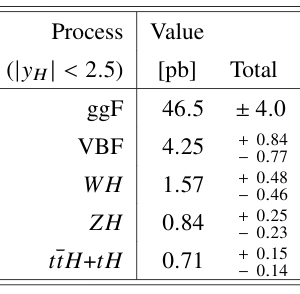
\includegraphics[width=\linewidth,height=0.5\textheight,keepaspectratio]{higgs_production_modes.png}
                \caption{source - arXiv:1909.02845 [hep-ex] }
            \end{figure}
        \end{column}
    \end{columns}
}


%\frame {
%    \begin{tikzpicture}
%      \begin{feynman}
%        \vertex (a);
%        \vertex [right=of a] (b);
%        \vertex [above=of a] (vb1);
%        \vertex [below=of a] (vb2);
%        \vertex [above left=of vb1] (q1i);
%        \vertex [below left=of vb2] (q2i);
%        \vertex [above right=of vb1] (q1f);
%        \vertex [below right=of vb2] (q2f);
%
%        \diagram* {
%            (q1i) -- (vb1) -- (q1f),
%            (q2i) -- (vb2) -- (q2f),
%            (vb1) -- [boson] (a) -- [boson] (vb2),
%            (a) -- [scalar] (b),
%        };
%      \end{feynman}
%    \end{tikzpicture}
%}





\frame {
    \frametitle{The Complication of Many Jets}
    %Show Ariel’s 3-jet scenario to illustrate logistical issues
    % Show your table of how common this is (~20%)
}
